\section{Introduction}
I have spent the majority of my time this week grasping the key ideas of Generative Adversarial from CVPR-2018\cite{cvpr18} and comparing the CVPR-2018 with CVPR-2017\cite{cvpr17} and ICCV-2017\cite{iccv17}.

\section{CVPR-2018}
Lecture videos could be found \href{https://www.youtube.com/playlist?list=PLvV9zfwRURxfydKkbFlyqn-GFsTY8-zRH}{here}.

This was a combination of multiple lectures:
\begin{enumerate}
\item Introduction to GAN\cite{gan} and SAGAN\cite{sagan}\cite{spectralnorm}
\item Paired Image-to-Image Translation\cite{pix2pix}\cite{pix2pixhd}
\item Unpaired Image-to-Image Translation with CycleGAN\cite{cyclegan}\cite{bicyclegan}
\item Do GANs learn the distribution?
\item Learning Disentangled Representations with an Adversarial Loss
\item VAE-GAN Hybrids
\item Multimodal Unsupervised Image-to-Image Translation
\item Adversarial Domain Adaptation
\item Adversaries for Detection and Action\cite{a-fast-rcnn}\cite{fast-rcnn}
\item Generative Adversarial Imitation Learning
\item Video Generation and Prediction
\end{enumerate}

I only captured new things compared to ICCV-2017 and CVPR-2017 about generative adversarial network and all of my taken note could be found here on my \href{https://github.com/tlvu2697/collection--generative-adversarial-network/tree/master/cvpr-18}{GitHub}.

\section{CycleGAN Demo}\cite{cyclegangithub}
\subsection{horse2zebra}

\newpage
\begin{figure}[!ht]
\centering
\begin{subfigure}{0.5\textwidth}
  \centering
  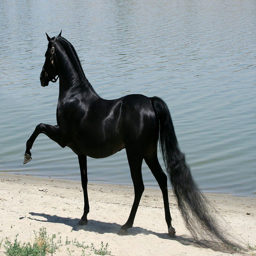
\includegraphics[height=0.25\textheight,keepaspectratio]{week7-black-horse-real-A.png}
  \caption{Input}
\end{subfigure}%
\begin{subfigure}{0.5\textwidth}
  \centering
  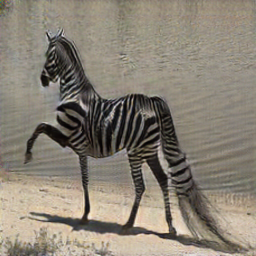
\includegraphics[height=0.25\textheight,keepaspectratio]{week7-black-horse-fake-B.png}
  \caption{Output}
\end{subfigure}
\caption{Horse to zebra with black horse}
\end{figure}
I thought this was an easy input for CycleGAN to deal with and the result was quite good although the background environment changed well, the horse's tail was not realistic at all.

\begin{figure}[!ht]
\centering
\begin{subfigure}{0.5\textwidth}
  \centering
  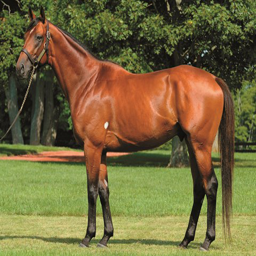
\includegraphics[height=0.25\textheight,keepaspectratio]{week7-brown-horse-real-A.png}
  \caption{Input}
\end{subfigure}%
\begin{subfigure}{0.5\textwidth}
  \centering
  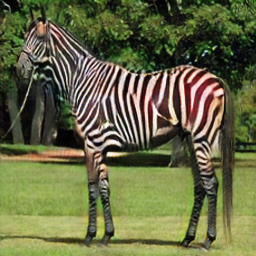
\includegraphics[height=0.25\textheight,keepaspectratio]{week7-brown-horse-fake-B.png}
  \caption{Output}
\end{subfigure}
\caption{Horse to zebra with brown horse}
\end{figure}
This test was extremely successful due to the correctness, the quality of the output. The results for this succeed maybe because the horse occupied most of the area of the input images and the pose of horse was really ideal.

\newpage
\begin{figure}[!ht]
\centering
\begin{subfigure}{0.5\textwidth}
  \centering
  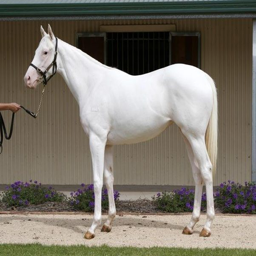
\includegraphics[height=0.25\textheight,keepaspectratio]{week7-white-horse-real-A.png}
  \caption{Input}
\end{subfigure}%
\begin{subfigure}{0.5\textwidth}
  \centering
  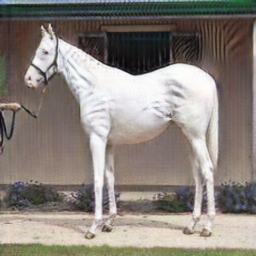
\includegraphics[height=0.25\textheight,keepaspectratio]{week7-white-horse-fake-B.png}
  \caption{Output}
\end{subfigure}
\caption{Horse to zebra with white horse}
\end{figure}
This test was failed. I did not know how to explain this case.

\subsection{zebra2horse}
\begin{figure}[!ht]
\centering
\begin{subfigure}{0.5\textwidth}
  \centering
  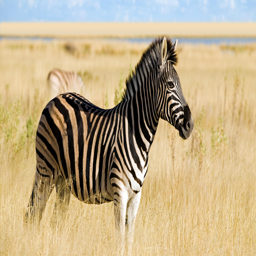
\includegraphics[height=0.25\textheight,keepaspectratio]{week7-zebra-1-real-A.png}
  \caption{Input}
\end{subfigure}%
\begin{subfigure}{0.5\textwidth}
  \centering
  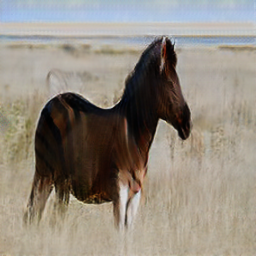
\includegraphics[height=0.25\textheight,keepaspectratio]{week7-zebra-1-fake-B.png}
  \caption{Output}
\end{subfigure}
\caption{Zebra to horse case 1}
\end{figure}
The generated horse was good, but one more time the background envi-ronment was significantly changed.

\newpage
\begin{figure}[!ht]
\centering
\begin{subfigure}{0.5\textwidth}
  \centering
  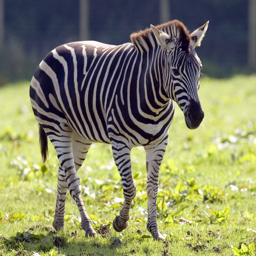
\includegraphics[height=0.25\textheight,keepaspectratio]{week7-zebra-2-real-A.png}
  \caption{Input}
\end{subfigure}%
\begin{subfigure}{0.5\textwidth}
  \centering
  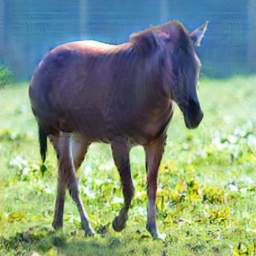
\includegraphics[height=0.25\textheight,keepaspectratio]{week7-zebra-2-fake-B.png}
  \caption{Output}
\end{subfigure}
\caption{Zebra to horse case 2}
\end{figure}
The environment background was also changed, the horse's color was good but its rear legs were weird.

\begin{figure}[!ht]
\centering
\begin{subfigure}{0.5\textwidth}
  \centering
  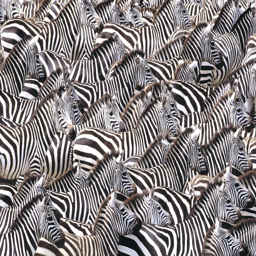
\includegraphics[height=0.25\textheight,keepaspectratio]{week7-zebra-3-real-A.png}
  \caption{Input}
\end{subfigure}%
\begin{subfigure}{0.5\textwidth}
  \centering
  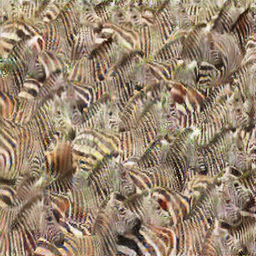
\includegraphics[height=0.25\textheight,keepaspectratio]{week7-zebra-3-fake-B.png}
  \caption{Output}
\end{subfigure}
\caption{Zebra to horse case 3}
\end{figure}
This input was too hard for CycleGAN and I was not surprised when Cygle-GAN was completely failed in this case.

\subsection{map2sat}
\newpage
\begin{figure}[!ht]
\centering
\begin{subfigure}{0.5\textwidth}
  \centering
  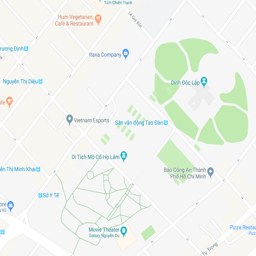
\includegraphics[height=0.25\textheight,keepaspectratio]{week7-map-real-A.png}
  \caption{Input}
\end{subfigure}%
\begin{subfigure}{0.5\textwidth}
  \centering
  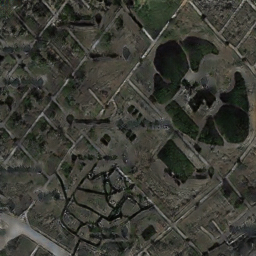
\includegraphics[height=0.25\textheight,keepaspectratio]{week7-map-fake-B.png}
  \caption{Output}
\end{subfigure}
\caption{Map to satellite}
\end{figure}
I did not find interesting in this model. The result was not good at all. It just replace the green part of the map by "tree" in the satellite, the white and yellow parts by "land". All of those stuffs were not impress me at all.

\subsection{sat2map}
\begin{figure}[!ht]
\centering
\begin{subfigure}{0.5\textwidth}
  \centering
  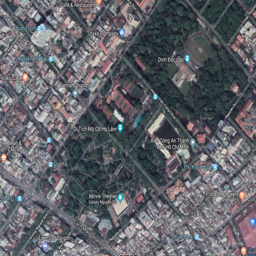
\includegraphics[height=0.25\textheight,keepaspectratio]{week7-sat-real-A.png}
  \caption{Input}
\end{subfigure}%
\begin{subfigure}{0.5\textwidth}
  \centering
  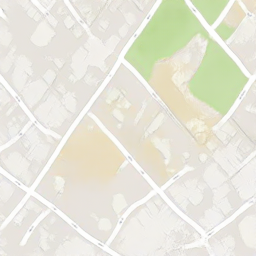
\includegraphics[height=0.25\textheight,keepaspectratio]{week7-sat-fake-B.png}
  \caption{Output}
\end{subfigure}
\caption{Satellite to map}
\end{figure}
This was a little bit better than the map2sat model, but I thought these two were still for entertaining purposes rather than serious situations in real life.

\subsection{style\_vangogh}
\newpage
\begin{figure}[!ht]
\centering
\begin{subfigure}{0.5\textwidth}
  \centering
  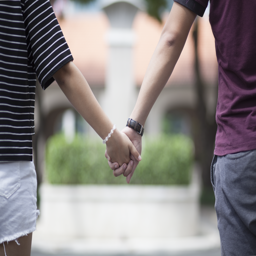
\includegraphics[height=0.25\textheight,keepaspectratio]{week7-vangogh-real-A.png}
  \caption{Input}
\end{subfigure}%
\begin{subfigure}{0.5\textwidth}
  \centering
  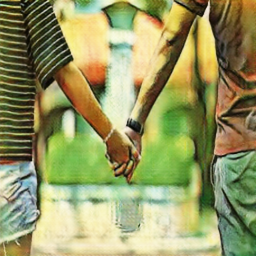
\includegraphics[height=0.25\textheight,keepaspectratio]{week7-vangogh-fake-B.png}
  \caption{Output}
\end{subfigure}
\caption{Vincent van Gogh style transfer}
\end{figure}
This paint was impressive, but I did not know such a thing about painting valuation so I could not tell whether this was Vincent van Gogh' styles or not.

\section{Image Style Transfer using CNN\cite{styletransfergithub}}
This repository was a TensorFlow implementation of Image Style Transfer using Convolutional Neural Networks\cite{styletransfer} and some other techniques\cite{styletransfervideo}\cite{preservingcolor}. The Neural Style algorithm synthesizes a pastiche by separating and combining the content of one image with the style of another image using Convolutional Neural Networks (CNN). These techniques were not supported or improved by GAN.

The content was one of my favorite pictures, the style image was \textbf{\emph{The Starry Night}}\cite{thestarrynight}. And the result was far from which I had imagined, it was so beautiful and high-detailed.

Watching this result I had a thought that why people need to "improve" the current CNN with GAN, the generated images' quality from GAN were much far from this.

\newpage
\begin{figure}[!ht]
\centering
\begin{subfigure}{\textwidth}
  \centering
  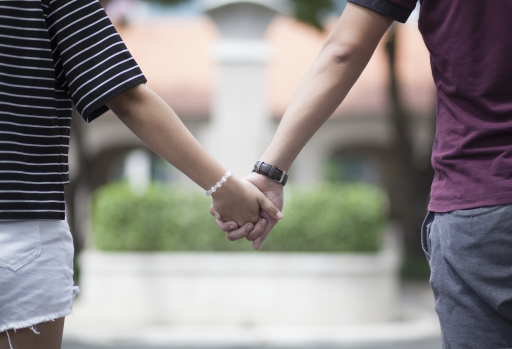
\includegraphics[height=0.25\textheight,keepaspectratio]{week7-styletransfer-content.png}
  \caption{Content}
\end{subfigure}
\begin{subfigure}{\textwidth}
  \centering
  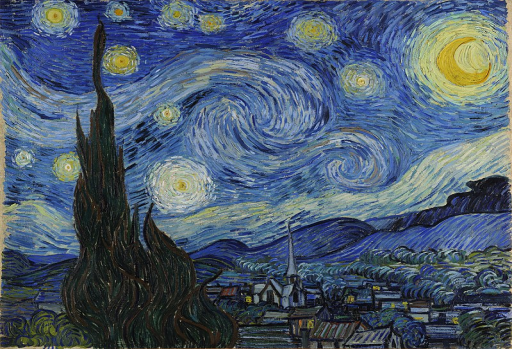
\includegraphics[height=0.25\textheight,keepaspectratio]{week7-styletransfer-style.png}
  \caption{Style}
\end{subfigure}
\begin{subfigure}{\textwidth}
  \centering
  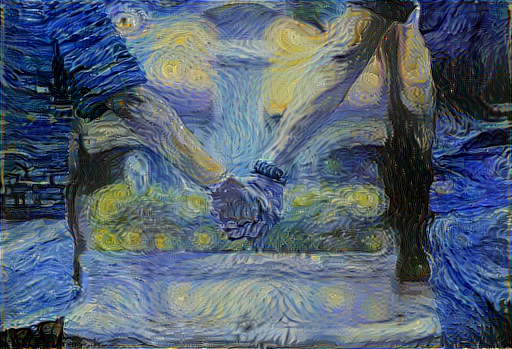
\includegraphics[height=0.25\textheight,keepaspectratio]{week7-styletransfer-result.png}
  \caption{Result}
\end{subfigure}
\caption{Style transfer with one input style}
\end{figure}